\documentclass[tikz,border=10pt]{standalone}
\usepackage{tikz}
\usetikzlibrary{positioning,shapes,arrows.meta,decorations.pathreplacing}

\begin{document}
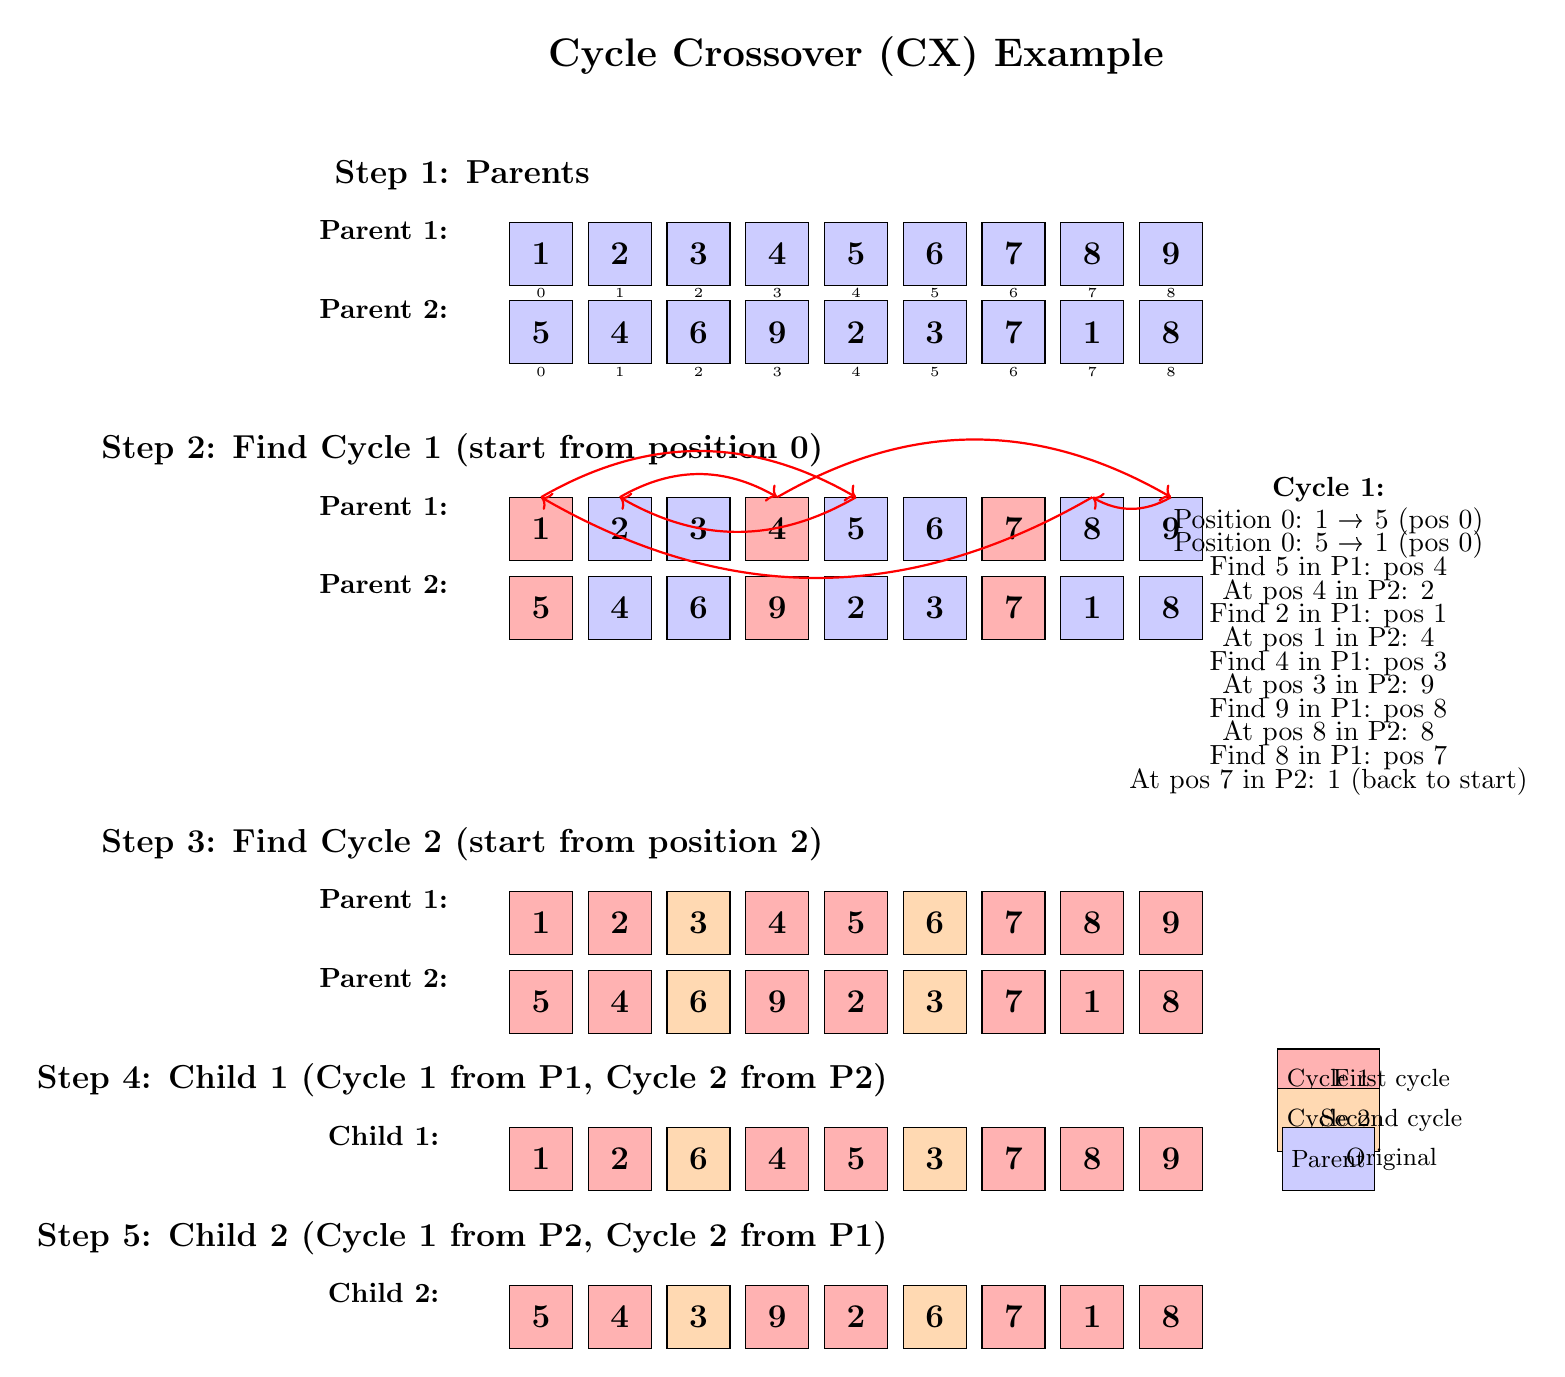
\begin{tikzpicture}[
    node distance=0.5cm,
    gene/.style={draw, rectangle, minimum width=0.8cm, minimum height=0.8cm, font=\large\bfseries},
    parent/.style={gene, fill=blue!20},
    child/.style={gene, fill=green!20},
    cycle1/.style={gene, fill=red!30},
    cycle2/.style={gene, fill=orange!30},
    cycle3/.style={gene, fill=purple!30},
    arrow/.style={->, thick, red}
]

% Title
\node[font=\Large\bfseries] at (4, 9) {Cycle Crossover (CX) Example};

% Step 1: Original Parents
\node[font=\large\bfseries] at (-1, 7.5) {Step 1: Parents};
\node[font=\bfseries] at (-2, 6.8) {Parent 1:};
\foreach \i/\val in {0/1, 1/2, 2/3, 3/4, 4/5, 5/6, 6/7, 7/8, 8/9} {
    \node[parent] (p1\i) at (\i, 6.5) {\val};
    \node[font=\tiny] at (\i, 6) {\i};
}

\node[font=\bfseries] at (-2, 5.8) {Parent 2:};
\foreach \i/\val in {0/5, 1/4, 2/6, 3/9, 4/2, 5/3, 6/7, 7/1, 8/8} {
    \node[parent] (p2\i) at (\i, 5.5) {\val};
    \node[font=\tiny] at (\i, 5) {\i};
}

% Step 2: Find Cycle 1
\node[font=\large\bfseries] at (-1, 4) {Step 2: Find Cycle 1 (start from position 0)};

\node[font=\bfseries] at (-2, 3.3) {Parent 1:};
\foreach \i/\val/\style in {0/1/cycle1, 1/2/parent, 2/3/parent, 3/4/cycle1, 4/5/parent, 5/6/parent, 6/7/cycle1, 7/8/parent, 8/9/parent} {
    \node[\style] (c1p1\i) at (\i, 3) {\val};
}

\node[font=\bfseries] at (-2, 2.3) {Parent 2:};
\foreach \i/\val/\style in {0/5/cycle1, 1/4/parent, 2/6/parent, 3/9/cycle1, 4/2/parent, 5/3/parent, 6/7/cycle1, 7/1/parent, 8/8/parent} {
    \node[\style] (c1p2\i) at (\i, 2) {\val};
}

% Cycle 1 explanation
\node[font=\bfseries] at (10, 3.5) {Cycle 1:};
\node[font=\normalsize] at (10, 3.1) {Position 0: 1 → 5 (pos 0)};
\node[font=\normalsize] at (10, 2.8) {Position 0: 5 → 1 (pos 0)};
\node[font=\normalsize] at (10, 2.5) {Find 5 in P1: pos 4};
\node[font=\normalsize] at (10, 2.2) {At pos 4 in P2: 2};
\node[font=\normalsize] at (10, 1.9) {Find 2 in P1: pos 1};
\node[font=\normalsize] at (10, 1.6) {At pos 1 in P2: 4};
\node[font=\normalsize] at (10, 1.3) {Find 4 in P1: pos 3};
\node[font=\normalsize] at (10, 1.0) {At pos 3 in P2: 9};
\node[font=\normalsize] at (10, 0.7) {Find 9 in P1: pos 8};
\node[font=\normalsize] at (10, 0.4) {At pos 8 in P2: 8};
\node[font=\normalsize] at (10, 0.1) {Find 8 in P1: pos 7};
\node[font=\normalsize] at (10, -0.2) {At pos 7 in P2: 1 (back to start)};

% Arrows showing cycle 1 connections
\draw[arrow, bend left=30] (c1p10.north) to (c1p14.north);
\draw[arrow, bend left=30] (c1p14.north) to (c1p11.north);
\draw[arrow, bend left=30] (c1p11.north) to (c1p13.north);
\draw[arrow, bend left=30] (c1p13.north) to (c1p18.north);
\draw[arrow, bend left=30] (c1p18.north) to (c1p17.north);
\draw[arrow, bend left=30] (c1p17.north) to (c1p10.north);

% Step 3: Find remaining cycles
\node[font=\large\bfseries] at (-1, -1) {Step 3: Find Cycle 2 (start from position 2)};

\node[font=\bfseries] at (-2, -1.7) {Parent 1:};
\foreach \i/\val/\style in {0/1/cycle1, 1/2/cycle1, 2/3/cycle2, 3/4/cycle1, 4/5/cycle1, 5/6/cycle2, 6/7/cycle1, 7/8/cycle1, 8/9/cycle1} {
    \node[\style] (c2p1\i) at (\i, -2) {\val};
}

\node[font=\bfseries] at (-2, -2.7) {Parent 2:};
\foreach \i/\val/\style in {0/5/cycle1, 1/4/cycle1, 2/6/cycle2, 3/9/cycle1, 4/2/cycle1, 5/3/cycle2, 6/7/cycle1, 7/1/cycle1, 8/8/cycle1} {
    \node[\style] (c2p2\i) at (\i, -3) {\val};
}

% Step 4: Create Child 1
\node[font=\large\bfseries] at (-1, -4) {Step 4: Child 1 (Cycle 1 from P1, Cycle 2 from P2)};

\node[font=\bfseries] at (-2, -4.7) {Child 1:};
\foreach \i/\val/\style in {0/1/cycle1, 1/2/cycle1, 2/6/cycle2, 3/4/cycle1, 4/5/cycle1, 5/3/cycle2, 6/7/cycle1, 7/8/cycle1, 8/9/cycle1} {
    \node[\style] (child1\i) at (\i, -5) {\val};
}

% Step 5: Create Child 2
\node[font=\large\bfseries] at (-1, -6) {Step 5: Child 2 (Cycle 1 from P2, Cycle 2 from P1)};

\node[font=\bfseries] at (-2, -6.7) {Child 2:};
\foreach \i/\val/\style in {0/5/cycle1, 1/4/cycle1, 2/3/cycle2, 3/9/cycle1, 4/2/cycle1, 5/6/cycle2, 6/7/cycle1, 7/1/cycle1, 8/8/cycle1} {
    \node[\style] (child2\i) at (\i, -7) {\val};
}

% Legend
\node[cycle1, font=\small] at (10, -4) {Cycle 1};
\node[cycle2, font=\small] at (10, -4.5) {Cycle 2};
\node[parent, font=\small] at (10, -5) {Parent};
\node[font=\small] at (10.8, -4) {First cycle};
\node[font=\small] at (10.8, -4.5) {Second cycle};
\node[font=\small] at (10.8, -5) {Original};

\end{tikzpicture}
\end{document}